

\documentclass[a4paper, 10pt]{dselReport}

\linespread{1.5}%设置行距为18pt
\hypersetup{colorlinks=true,linkcolor=black}%设置目录超链接方式




%%%% 正文开始 %%%%
\begin{document}


%%%% 定义标题格式,包括title,author,affiliation,email等 %%%%
\title{深空探测实验室\LaTeX 模板 \\ \subtitle{月球大工程} }



\author{净整没用的
\footnote{电子邮件: jingzhengmeiyongde@dsel.mail.com}\\[4ex]
}
\date{2023年12月}


\CKeyword{关键词1;关键词2;}%填入关键词


%%%% 以下部分是正文 %%%%  
\maketitle

\newpage
\thispagestyle {empty}  %设置空白页,并删除页眉页脚
\mbox{}
\newpage

\newpage
\begin{abstract}
美国陆军部于1942年6月开始实施利用核裂变反应来研制原子弹的计划,亦称曼哈顿计划(Manhattan Project)。该工程集中了当时西方国家(除纳粹德国外)最优秀的核科学家,动员了10万多人参加这一工程,历时3年,耗资20亿美元,于1945年7月16日成功地进行了世界上第一次核爆炸,并按计划制造出两颗实用的原子弹。整个工程取得圆满成功。在工程执行过程中,负责人L.R.格罗夫斯和R.奥本海默应用了系统工程的思路和方法,大大缩短了工程所耗时间。这一工程的成功促进了第二次世界大战后系统工程的发展。
\end{abstract}

{\hei\sihao \makebox{关键词}:} \avicitCKeyword


%%%% 以下部分为前言, 请替换 相应文字 %%%%  
\newpage
\setcounter{page}{1}

\begin{center}
    \sanhao\hei{前言}
\end{center}~\

这是前言部分.

强化 细化 深化

打造 建造 创造 

\newpage


%%%% 以下部分为正文内容, 请替换 相应文字 %%%%  
\newpage
\begin{center}
\tableofcontents
\end{center}
\newpage

\section{文字}
Latex内容基本分为文字和命令两部分。正常文字输出会按照模板cls文件的规定排版,而命令的总是以反斜杠$\backslash$ 开始,勇于特殊符号的输入,或者插入图片表格等。下文中为基本文字: 

到1941年12月6日,美国正式制定了代号为“曼哈顿”的绝密计划。 罗斯福总统赋予这一计划以“高于一切行动的特别优先权”。

1937年2月,纳粹德国开始执行了“铀计划”。1941年末,珍珠港事件后,美国参加了二次大战,与纳粹德国宣战。一些美国科学家提议要先于纳粹德国制造出原子弹。
例如爱因斯坦给罗斯福的原信如下:
Albert Einstein
Old Grove Rd.
Nassau Point

这些文字中,空行表示另起一段。



\subsection{图片插入}
图片格式兼容性很高,推荐使用eps图片。 如果是用Microsoft Visio做的流程图,可以保存成pdf之后当成图片插入。


\begin{figure}[ht!]
\centering
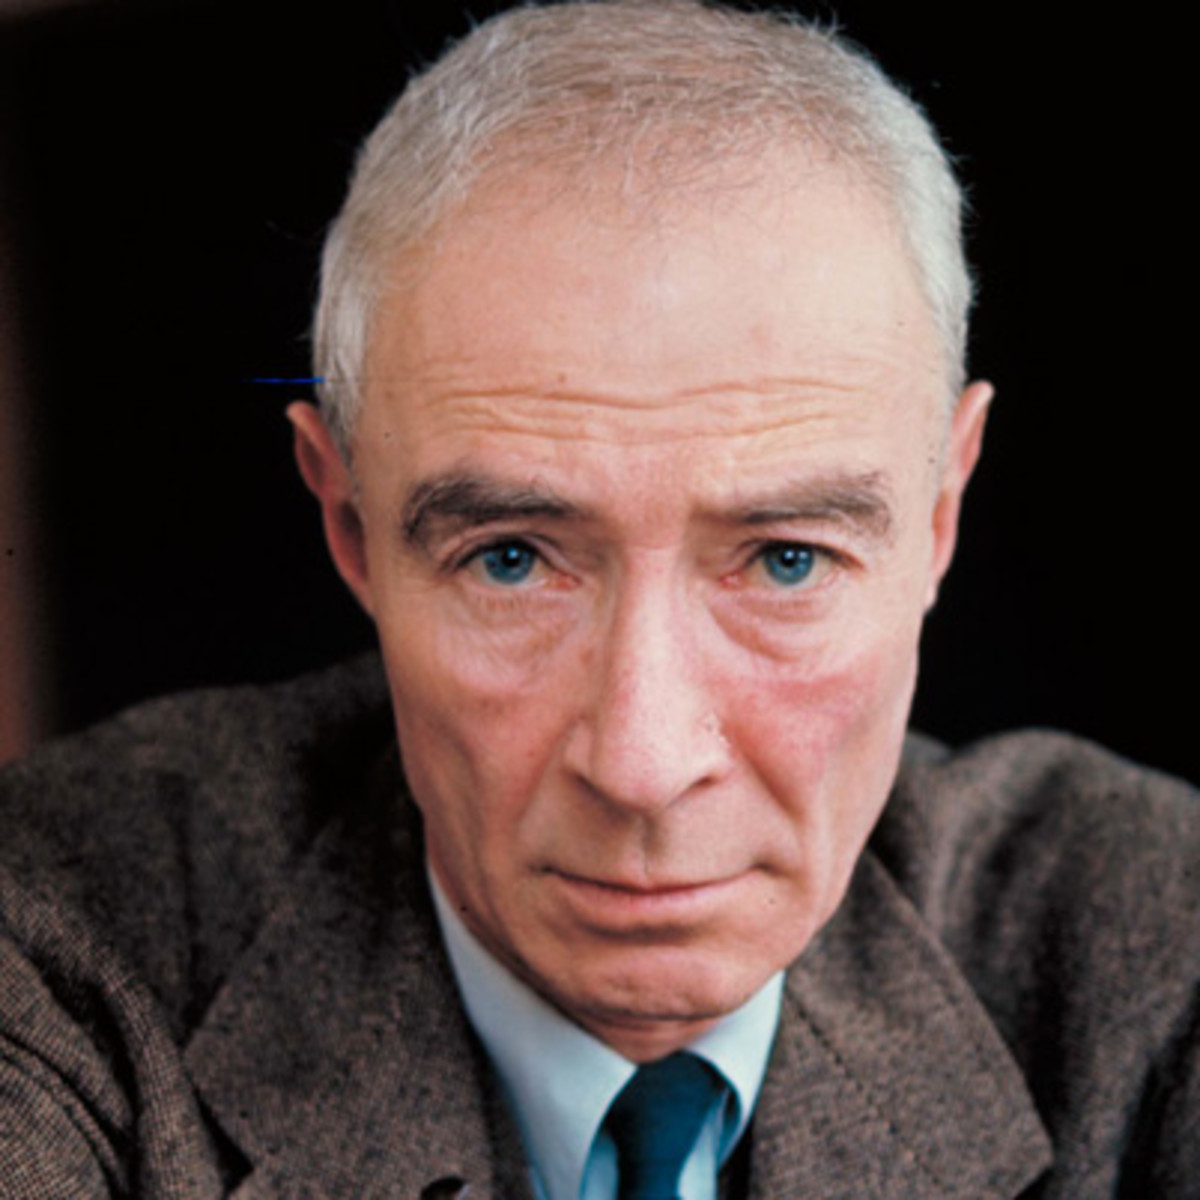
\includegraphics [scale=0.2,trim=0 0 0 0]{aobenhai.jpg}%输入本文件夹内的图片名称
\caption{奥本海本人照片}%图片描述
\label{fig1}%图片的label
\end{figure}


图片会自动加上需要,在图片设置中可以加上label,方便在文中其他地方引用,引用命令为ref。 比如图片\ref{fig1}展示的是奥本海本人。


上面插入图片的源代码为:
\begin{lstlisting}
\begin{figure}[ht!]
\centering
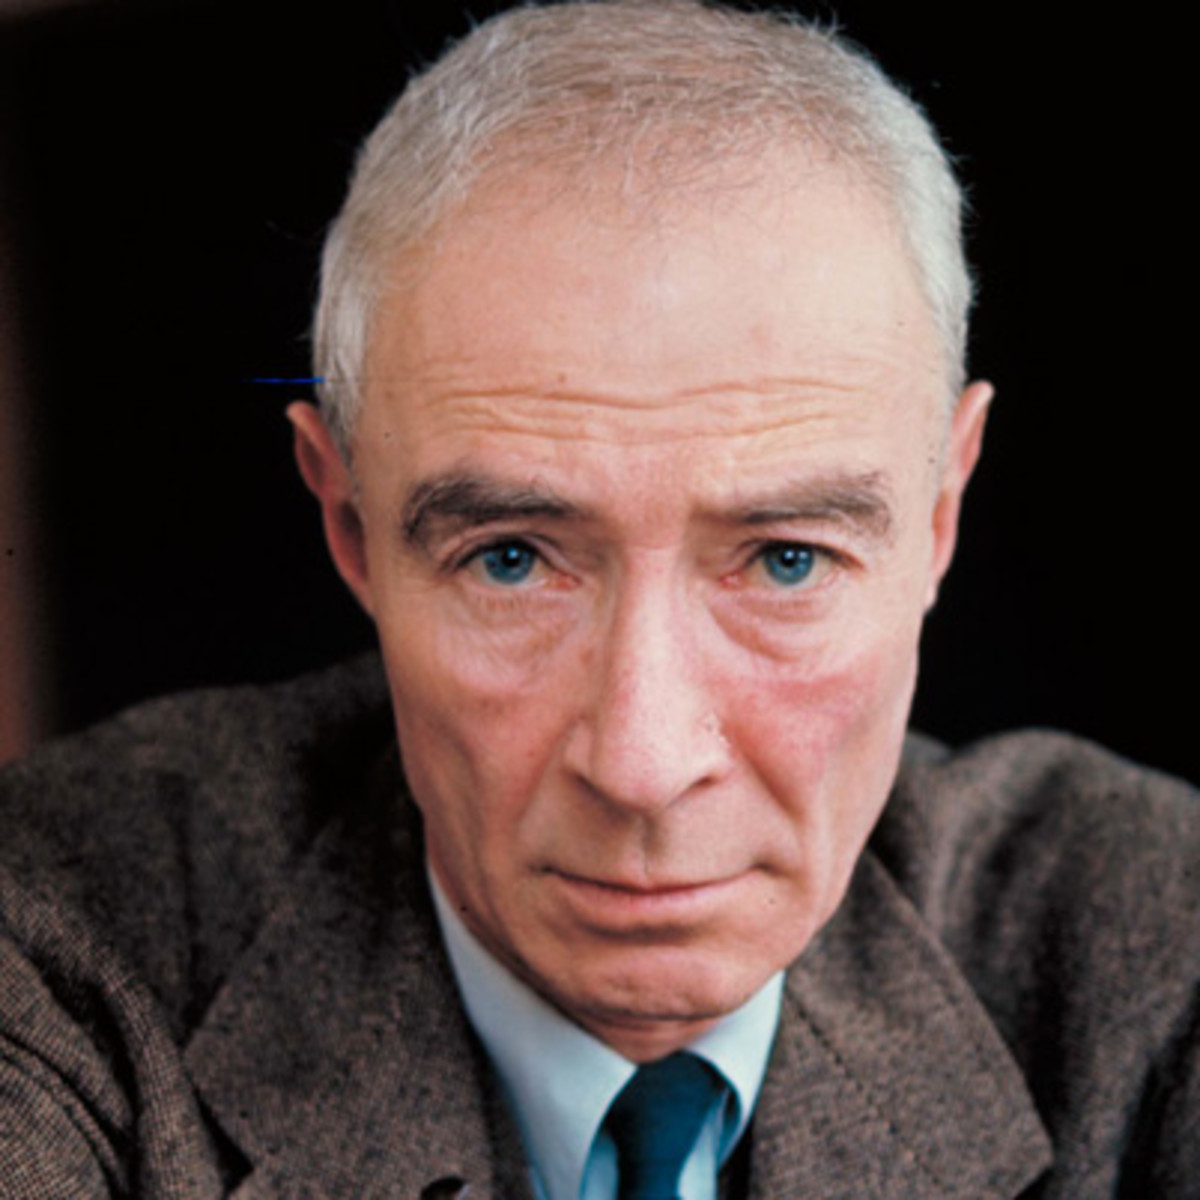
\includegraphics [scale=0.2,trim=0 0 0 0]{aobenhai.jpg}%输入本文件夹内的图片名称
\caption{奥本海本人照片}%图片描述
\label{fig1}%图片的label
\end{figure}
\end{lstlisting}

可以看出只要输入图片的名称和图片的描述文字就可以了。


\subsubsection{表格插入}

\begin{table}[h]
\centering
\captiontitlefont{\xiaowuhao\bf }%图或者表格内部都可以重新定义字体
\caption{传输线积冰条件}%表格文字说明
\begin{tabular}{cccc}%四列,四个c
\toprule %横线
{编号} &  {直径}/\si{\metre} & {静温}/\si{\kelvin} & {时间}/min\\
\midrule %横线
4 & 0.0349 & 268.15 & 30\\ %内容用&符号分割, 最后\\表示换行
5 & 0.01905 & 268.15 & 30\\
\bottomrule%横线
\end{tabular}
\end{table}

上文中表格的源代码为:

\begin{lstlisting}
\begin{table}[h]
\centering
\captiontitlefont{\xiaowuhao\bf }%图或者表格内部都可以重新定义字体
\caption{传输线积冰条件}%表格文字说明
\begin{tabular}{cccc}%四列,四个c
\toprule %横线
{编号} &  {直径}/\si{\metre} & {静温}/\si{\kelvin} & {时间}/min\\
\midrule %横线
4 & 0.0349 & 268.15 & 30\\ %内容用&符号分割, 最后\\表示换行
5 & 0.01905 & 268.15 & 30\\
\bottomrule%横线
\end{tabular}
\end{table}
\end{lstlisting}

\section{公式编辑}
Latex拥有最强的公式编辑能力, 其公式完全用代码写成,简单优雅,没有二义性。

\begin{equation}
\lim_{x \to \infty} x^2_{22} - \int_{1}^{5}x\mathrm{d}x + \sum_{n=1}^{20} n^{2} = \prod_{j=1}^{3} y_{j}  + \lim_{x \to -2} \frac{x-2}{x}
\end{equation}


公式的源代码为:
\begin{lstlisting}
\begin{equation}
\lim_{x \to \infty} x^2_{22} - \int_{1}^{5}x\mathrm{d}x + \sum_{n=1}^{20} n^{2} = \prod_{j=1}^{3} y_{j}  + \lim_{x \to -2} \frac{x-2}{x}
\end{equation}
\end{lstlisting}

不要被这些复杂的符号吓到, 只要查看符号列表,就会发现其掌握难度都低于脚本语言。



\section{插入源代码}
有时候我们需要插入一些源代码,或者伪代码,比如:
\begin{lstlisting}
#include<iostream>
using namespace std;
 
 
int main() {
 
    double choice = 0;
    double choice1 = 0;
    double choice2 = 0;
    double choice3 = 0;
    double choice4 = 0;
     
    FLAG:
    cout << "请输入需要计算的类型" << endl;
    cout << "1.面积" << endl;
    cout << "2.体积" << endl;
    cout << "3.表面积" << endl;
    cout << "4.周长" << endl;
 
    cin >> choice;
    if (choice == 1)
    {//面积
        cout << "请输入需要计算的图形" << endl;
        cout << "1.正方形" << endl;
        cout << "2.长方形" << endl;
        cout << "3.圆形" << endl;
        cout << "4.平行四边形" << endl;
        cout << "5.梯形" << endl;
        cout << "6.三角形形" << endl;
        cin >> choice1;
        if (choice1 == 1) //正方形的面积
        {
            cout << "请输入正方形的边长" << endl;
            double Sidelength = 0;
        }
    }
    else
    {
        cout << "输入错误,请重新输入" << endl;
        goto FLAG;
    }
 
    system("pause");
 
    return 0;
}
\end{lstlisting}


使用"$\backslash$begin{lstlisting}+ 代码内容 + $\backslash$end{lstlisting}"就可以高亮显示代码,本模板已经为大家设置好了C++语言环境。


和C++一样,Latex中的大括号\{\}都有作用域的功能:

{\erhao\kai{\color{red}{You Are Welcome!}}}






\section{插入参考文献}
参考文献的插入和使用在Latex中非常简单,基本上只需要将网上的文章信息下载后粘贴到tex文件中就可以。

比如本文之后的参考文献的源代码就是:

\begin{lstlisting}

\begin{thebibliography}{100}%最多添加100个参考文献,可以自己修改

\bibitem{ref1}郭莉莉,白国君,尹泽成,魏惠芳. “互联网+”背景下沈阳智慧交通系统发展对策建议[A]. 中共沈阳市委、沈阳市人民政府.第十七届沈阳科学学术年会论文集[C].中共沈阳市委、沈阳市人民政府:沈阳市科学技术协会,2020:4.
\bibitem{ref2}陈香敏,魏伟,吴莹. “文化+人工智能”视阈下文化创意产业融合发展实践及路径研究[A]. 中共沈阳市委、沈阳市人民政府.第十七届沈阳科学学术年会论文集[C].中共沈阳市委、沈阳市人民政府:沈阳市科学技术协会,2020:4.
\bibitem{ref3}田晓曦,刘振鹏,彭宝权. 地方高校开展教育人工智能深度融合的路径探究[A]. 中共沈阳市委、沈阳市人民政府.第十七届沈阳科学学术年会论文集[C].中共沈阳市委、沈阳市人民政府:沈阳市科学技术协会,2020:5.
\bibitem{ref4}柏卓君,潘勇,李仲余.彩色多普勒超声在早期胚胎停育诊断中的应用[J].影像研究与医学应用,2020,4(18):129-131.
\bibitem{ref5}杨芸.我院2018年人血白蛋白临床应用调查与分析[J].上海医药,2020,41(17):34-35+74.

\end{thebibliography}

\end{lstlisting}

我们推荐google学术搜索文章得到的参考文献标识,其规范,专业。引用文献和引用图片表格的方式近似,但是需要使用的$\backslash$cite $\backslash$citet $\backslash$citep 命令,至于三者有什么不同? 不妨自己试试看?




\begin{thebibliography}{100}

\bibitem{ref1}郭莉莉,白国君,尹泽成,魏惠芳. “互联网+”背景下沈阳智慧交通系统发展对策建议[A]. 中共沈阳市委、沈阳市人民政府.第十七届沈阳科学学术年会论文集[C].中共沈阳市委、沈阳市人民政府:沈阳市科学技术协会,2020:4.
\bibitem{ref2}陈香敏,魏伟,吴莹. “文化+人工智能”视阈下文化创意产业融合发展实践及路径研究[A]. 中共沈阳市委、沈阳市人民政府.第十七届沈阳科学学术年会论文集[C].中共沈阳市委、沈阳市人民政府:沈阳市科学技术协会,2020:4.
\bibitem{ref3}田晓曦,刘振鹏,彭宝权. 地方高校开展教育人工智能深度融合的路径探究[A]. 中共沈阳市委、沈阳市人民政府.第十七届沈阳科学学术年会论文集[C].中共沈阳市委、沈阳市人民政府:沈阳市科学技术协会,2020:5.
\bibitem{ref4}柏卓君,潘勇,李仲余.彩色多普勒超声在早期胚胎停育诊断中的应用[J].影像研究与医学应用,2020,4(18):129-131.
\bibitem{ref5}杨芸.我院2018年人血白蛋白临床应用调查与分析[J].上海医药,2020,41(17):34-35+74.

\end{thebibliography}



\newpage
\vspace{1em}
{\hei\wuhao 致谢\quad}
{\fang\wuhao 
(如果有需要)

感谢某某……注意:首页注明基金项目后,文末不必再致谢。
}


\vskip 20pt
 
 \noindent {\hei 附录A:(如果有需要)}
 
若确有特殊需要设附录的,附录部分置于作
者简介后,标题为“附录A:”、“附录B:”......。公式
用大写字母和数字顺序编号,例如“(A1)”, “(A2)”。




\end{document}